%!TEX root = thesis.tex

\newcommand{\TheTitle}{Sensitivities of Porous Beds and Plates to Ignition by Firebrands}
\renewcommand{\TheAuthors}{Derek Bean, David L. Blunck}

\newcommand{\TheAddress}{
\textit{Frontiers in Mechanical Engineering} \\
Vol.~7, 1-11, 2021. \\
\doi{10.3389/fmech.2021.653810}
}

\PaperHeader{\TheTitle}{\TheAuthors}{\TheAddress}

\chapter{\TheTitle}
\label{part:manuscript1}

\section{Abstract}
    The increasing occurrence of severe wildfires, coupled with the expansion of the wildland urban interface has increased the number of structures in danger of being destroyed by wildfires. Ignition by firebrands is a significant avenue for fire spread and structure loss; thus, understanding processes and parameters that control the ignition of fuel beds by firebrands is important for reducing these losses. In this study the effect of fuel bed characteristics (i.e., particle size and porous or solid fuel bed) on ignition behavior was considered.  Modelling and analysis was conducted to better understand parameters that are dominant in controlling ignition. The fuel beds, made from Douglas-fir shavings, Douglas-fir plates, or cardboard plates, were heated with a cartridge heater (i.e., surrogate firebrand) to observe ignition. Smaller particles were observed to ignite more readily in porous beds than larger particles when heat transfer from the heater is primarily through conduction. This occurs in large part due to differences in contact area between the fuel bed and the heater coupled  with thermal properties of the fuel bed. As particle sizes increased, ignition was more likely to occur at extended times (\textgreater 100\si{\second}) due to the increased importance of radiation heat transfer. Douglas-fir plates were primarily observed to ignite at times where conduction was the dominant mode of heat transfer (\textless 10\si{\second}). Heat flux delivered to the fuel bed was observed to be a more accurate predictor of ignition likelihood and ignition time than heater temperatures. The characteristic ratio of transport and chemical timescales can be used, in conjunction with the measured heat flux and thermal diffusivity of the fuel beds, as a first approximation to predict ignition for the porous fuel beds. This suggests that future work focusing on these parameters may produce a general characterization of fuel bed ignition probability across fuel beds materials and morphologies.  

\section{Introduction}
     Increasing urban expansion into the wilderness has increased the area of the wildland urban interface (WUI). The increase of the WUI, coupled with global climate change has resulted in fires of increasing severity, size, and impact to humans. For example, consider the state of California in the United States, where four of the five largest fires and three of the five most destructive fires have occurred in the past decade~\cite{CalFire2019, CALFIRE2018}. These fires highlight a trend in the increasing severity of wildfires. Of particular concern with the increasing severity of wildfires is the severity of fires in the WUI. The 2018 Camp fire, where residential property losses amounted to more than twice the reported costs for nationwide federal suppression efforts during the same year~\cite{USDOI/USDA2019, Insurance2019}, is a stark example of how severe a fire that occurs in the WUI can be. A significant mechanism for the spread of fires into the WUI, or even within the WUI, is the ignition of fuel beds by firebrands~\cite{Mell2010, Maranghides2013NISTIgnitions}. Ignition by firebrands in wildfires occurs when a hot combusting particle is generated within the fire and transported, typically by wind, to a recipient fuel bed~\cite{Koo2010a}. Structures in the WUI often have geometry conducive to the collection of firebrands, further increasing the risk of ignition~\cite{Suzuki2020}. Hence, efforts to mitigate the destruction that can be caused by fires in the WUI must consider the role of ignition by firebrands.
     
    Three primary processes control the ignition of fuel beds by firebrands. Specifically, heat transfer between the fuel bed and the firebrand, pyrolyzate generation in the fuel bed, and the mixing of the pyrolyzates above the bed at sufficient temperatures for ignition to occur \cite{Babrauskas2003}. A recent review of the role of firebrands in the spread of fires by Manzello et al.~\cite{Manzello2020} identified that research into the ignition behavior of fuel beds by firebrands is critical to improving preventative measures. Work conducted by Manzello et al.~\cite{Manzello2006a, Manzello2006, Manzello2008} studying ignition of various fuel bed materials (e.g., cut grass and pine needle beds) concluded that the most influential factors for ignition were the number flux of firebrands to the fuel bed, the size of the firebrands, and the airflow over the fuel bed. Similar conclusions were found by Urban et al.~\cite{Urban2019a}, who found that larger firebrands were more likely to ignite fuel beds (i.e., fine sawdust) across a range of fuel moisture contents. These observations illustrate the critical role of heat transfer to the fuel bed in causing ignition. What is not clear from studies such as these is how ignition behavior would change for fuel beds other than those tested, even if identical firebrands were used. Even how the size of fuel particles alter ignition is not clear. Such knowledge is needed to help transition knowledge to a variety of fuel beds that can be present near the WUI (e.g., wood shavings, needles, leaves, etc.). 
    
    Essential to understanding the ignitablility of fuel beds is understanding how the role of heat transfer and energy of a firebrand influences ignition. Hadden et al.~\cite{Hadden2011} found that as the energy content of hot metal particles increased the ignition probability increased. It was also observed that the particle energy alone is not a sufficient condition for ignition to occur and that a minimum particle temperature is required. Similarly, Zak et al.~\cite{Zak2014} observed that the energy of a metal particle was not a sufficient parameter for ignition and minimum values for particle energy and temperature are required; the values of which are dictated by the ability of hot particles to generate sufficient amounts of hot pyrolyzates in fuel beds. Further studies by Fernandez-Pello et al.~\cite{Fernandez-Pello2015} added to the understanding of these factors concluding that heat losses from the hot particle, which reduce the heat flux to the fuel bed, can have a significant impact on the ignition of fuel beds. Additional studies conducted by Urban et al.~\cite{Urban2017, Urban2018} found that the timescale of flaming ignition can be relatively short ($\le$ 100 ms).  Furthermore, smaller fuel bed particles tended to ignite at lower metal particle temperatures. A sensitivity of ignition to the chemical composition of the fuel bed was also observed. While sensitivities to fuel bed particle size, ember particle size, and ember energy have been observed, the relative effect of each parameter on ignition limits and a general application of these sensitivities across various fuel beds and embers remains elusive. 
    
    Studies evaluating the heat flux of firebrands and the critical heat flux for ignition have yielded further insights into the ignition process. Hakes et al.~\cite{Hakes2019a} found that, for a single cylindrical firebrand and piles of firebrands, peak heat flux values ranged between 20 and 60 \si{\kilo\watt\per\square\meter} with average heat fluxes between 12 and 25 \si{\kilo\watt\per\square\meter}. The mass of the firebrands or piles of firebrands had little effect on the peak heat flux but directly influenced the total energy released. Tao et al.~\cite{Tao2020} observed similar heat fluxes for various of natural and manufactured firebrands. Both Hakes et al.~\cite{Hakes2019a} and Tao et al.~\cite{Tao2020} observed that an increase in wind speed significantly increased the measured heat flux. Hernandez et al.~\cite{Hernandez2017} found that Monterey Pine (\textit{pinus radiata}) needles ignited under heat flux as low as 10 \si{\kilo\watt\per\square\meter} with ignition time decreasing proportionally to the inverse square of increasing heat flux. In similar tests but with different fuels, Rivera et al.~\cite{Rivera2020} observed that critical heat fluxes for ignition were highly dependent on fuel bed properties with the critical radiative heat flux increasing as the porosity decreased. Reported critical values ranged from 6.64 \si{\kilo\watt\per\square\meter} to 20.85\si{\kilo\watt\per\square\meter} for Monterey Pine needles with porosities of 0.09 and 0.01, respectively. It has been observed that a variety of firebrands are capable of producing heat fluxes well above the critical heat flux values long enough for ignition in some fuels. However, upon comparing these values to other studies, ignition is not guaranteed if the critical heat flux rate and duration are met. For example, experiments conducted by Manzello et al.~\cite{Manzello2008} used firebrands similar to Hakes et al.~\cite{Hakes2019a} and Tao et al.~\cite{Tao2020} with fuels similar to Hernandez et al.~\cite{Hernandez2017} and Rivera et al.~\cite{Rivera2020} (e.g., wooden disks on pine needles) but did not observe ignition under conditions that would be anticipated to produce ignition. It should be noted that the studies conducted by Hernandez et al. and Rivera et al. were conducted under quiescent conditions and those by Manzello et al. between 0.5\si{\meter\per\second} and 1.0\si{\meter\per\second}. Nevertheless, the reported values of firebrand heat flux at 0.5\si{\meter\per\second} and 1.2\si{\meter\per\second} conditions by Tao et al. suggest ignition is likely to occur for instances where no ignition was observed. Not observing ignition under conditions at the apparent intersection of these findings suggests that other factors may be as important as heat flux and duration of heating. 

    Given this background and motivation the objective of this work is to identify how the size of fuel particles influences ignition and to ascertain changes in ignition of porous and solid fuels. Time to ignition tests with a cartridge heater were conducted to elucidate this sensitivity. It is anticipated that the observations from this study will enhance the understanding of fuel bed ignition and enable more focused studies regarding additional effects of fuel bed properties on ignition. 
  
 
\section{Methodology}
   The time to ignition was measured for five different fuel bed conditions with varying surface temperatures of a resistance heater.  The time to ignition was the metric used to evaluate the ignition propensity. The experimental apparatus, as illustrated in Figure~\ref{fig:ignPropensity}, was designed to replicate both conduction and radiation that may occur when a firebrand lands on the fuel bed. The heater was held in place by a lever arm that, when lowered, positioned the heater at a fixed location for the duration of the test. The firebrand was represented by a 6.35\si{\milli\meter} diameter 51\si{\milli\meter} long cartridge heater capable of a 250\si{\watt} output. The heater was inserted 3\si{\milli\meter} into the bed (approximately half the diameter) in the porous media tests and on top of the plates for the other experiments. The temperature of the heater was continually recorded via a type-K thermocouple attached to the top of the heater. An important distinction between using the lever arm holder and a naturally occurring firebrand is that the location of the heater remained fixed and, for times greater than roughly 10\si{\second}, could lose contact with the fuel bed as material was lost because of pyrolysis.  Thus, for the longer ignition experiments the arrangement mimicked a firebrand with a gap between it and the fuel bed, instead of a firebrand that maintained consistent contact. The rationale in using the lever arm was to ensure that the heater was placed a consistent depth within the fuel bed since sensitivities of ignition to heat source penetration depth have been observed by Wang et al.~\cite{Wang2016}. The temperature of the heater was held to within $\pm$ 6\% of the set point using PID control implemented in LabVIEW. Power delivery to the heater was measured at a rate of 1kHz for all tests. 
   Admittedly, the temperature and heat transfer from an actual firebrand to a fuel bed may vary more than that of a controlled heater, nor does the heater have a piloted ignition source. Nonetheless, trends of ignition propensity are expected to be similar between the heater and firebrands since the heat transfer rates calculated in these experiments are in the range of 1\si{\kilo\watt\per\square\meter} to 21\si{\kilo\watt\per\square\meter} which are comparable to heat flux values reported by Hakes et al.~\cite{Hakes2019a} and Tao et al.~\cite{Tao2020} for combustion of glowing firebrands on an instrumented surface. The advantage of using a heater was that it allowed sensitivities of ignition to the fuel beds and controlling processes to more readily be identified because the boundary conditions were measured, controlled, and consistent.
   
    Wood particles and flat plates were used as the fuel bed materials. The fuel particles were Douglas-fir (\textit{Pseudotsuga menziesii}) shavings sorted into three size classes: $L_{c}<$1\si{\milli\meter}, 4\si{\milli\meter} $<L_{c}<$ 6\si{\milli\meter}, and 6\si{\milli\meter} $<L_{c}<$ 12\si{\milli\meter} to allow sensitivities of ignition to be identified. Fuel particles were generated by processing Douglas-fir lumber through a planer and then sorted by screening and/or granulating to achieve the desired size distribution. The fuels were placed in a glass container with a diameter 140\si{\milli\meter} and a depth of 70\si{\milli\meter}. The container was filled to the rim for the porous media tests, but the fuels were not packed. The materials used for the tests with flat plates were Douglas-fir and corrugated cardboard processed into 75\si{\milli\meter}-by-75\si{\milli\meter} squares. The thickness of the Douglas-fir and cardboard plates were 5\si{\milli\meter} and 6\si{\milli\meter} respectively. For plate ignition tests, the plates were stacked in the container to be level with the rim, replicating the porous media tests as close as possible.
   
    The time to ignition was determined from the signal emitted from a BPX65 photodiode positioned to capture the lowering of the cartridge heater and the flames resulting from ignition. This measurement approach only considered flaming ignition. The time to ignition was defined as the time between the maximum light intensity gradients, which corresponds to lowering the heater onto the fuel bed and the ignition event. The photodiode was sampled at 1kHz. Consistency in airflow, and thus oxygen availability, was achieved by maintaining the apparatus in the same orientation in a fume hood with the same airflow settings for every test. The average air velocity over the fuel bed was measured using a hot wire anemometer (TSI IFA300). Measurements were taken with the sample bowl filled with fuel particles and the heater in the lowered testing position at room temperature with the probe positioned approximately 16\si{\milli\meter} above the fuel bed. The average air velocity over the fuel bed was 0.1\si{\meter\per\second}.
        \begin{figure}[htpb]
            \centering
            \resizebox{\figureWidthSet}{!}{%
            \begin{tikzpicture}
                \filldraw [draw=black!60, pattern=north west lines, pattern color= brown] (0, 0) rectangle (140mm, 70mm) node[pos=0.5, fill=white] {\Huge Fuel Bed}; 
                \filldraw[] (0mm, -2mm) rectangle (140mm,0mm) node[rotate=-90, pos=0.5] {};
                \filldraw[] (-2mm, -2mm) rectangle (0mm,70mm) node[rotate=-90, pos=0.5] {};
                \filldraw[] (140mm, 70mm) rectangle (142mm,-2mm) node[rotate=-90, pos=0.5] {};
                \filldraw [fill=red, draw=black] (45mm, 67mm) rectangle (95mm, 73mm) {}; 
                \filldraw [draw=black, fill=black!50] (55mm, 65mm) rectangle (58mm, 85mm) {};
                \filldraw [draw=black, fill=black!50] (66mm, 85mm) rectangle (48mm, 185mm) {};
                \filldraw [draw=black, fill=black!50] (-85mm, 220mm) rectangle (-67mm, -2mm) {};
                \filldraw [draw=black, fill=black!50, rotate around={-15:(57mm, 100mm)}] (66mm, 95mm) rectangle (-100mm, 105mm) {};
                \filldraw [draw=black, fill=black!50, rotate around={-15:(57mm, 170mm)}] (66mm, 165mm) rectangle (-100mm, 175mm) {};
                \filldraw [draw=black, fill=black!50] (-90mm, -2mm) rectangle (150mm, -4mm) {};
                \filldraw (57mm, 170mm) circle (2mm);
                \filldraw (57mm, 100mm) circle (2mm);
                \filldraw (-76mm, 205mm) circle (2mm);
                \filldraw (-76mm, 135mm) circle (2mm);
                \filldraw [rotate around={15:(140mm, 85mm)}] (140mm, 85mm) rectangle (145mm, 90mm) node[above right] {\Huge Photodiode};
                \draw [<-, line width=1mm] (75mm, 75mm) -- (125mm, 120mm) node[right] {\Huge Heater};
                \draw [dashed] (140mm, 87.5mm) -- (100mm, 72mm);
                \draw [dashed] (140mm, 87.5mm) -- (80mm, 74mm);
            \end{tikzpicture}
            }
            \caption{Experimental apparatus for the ignition propensity tests. The lever arm used to lower the apparatus into the fuel bed, the fuel bed size relative to the heater, and the location of the photodiode are illustrated.}
            \label{fig:ignPropensity}
        \end{figure}

        % An example photodiode trace is shown in Figure~\ref{fig:photoTrace} where the raw signal, the filtered signal, and the gradient of the filtered signal are shown. 
        % \begin{figure}[htbp]
        %     \begin{center}
        %     \begin{tikzpicture}
        %     \node[anchor=south west,inner sep=0] (image) at (0,0) {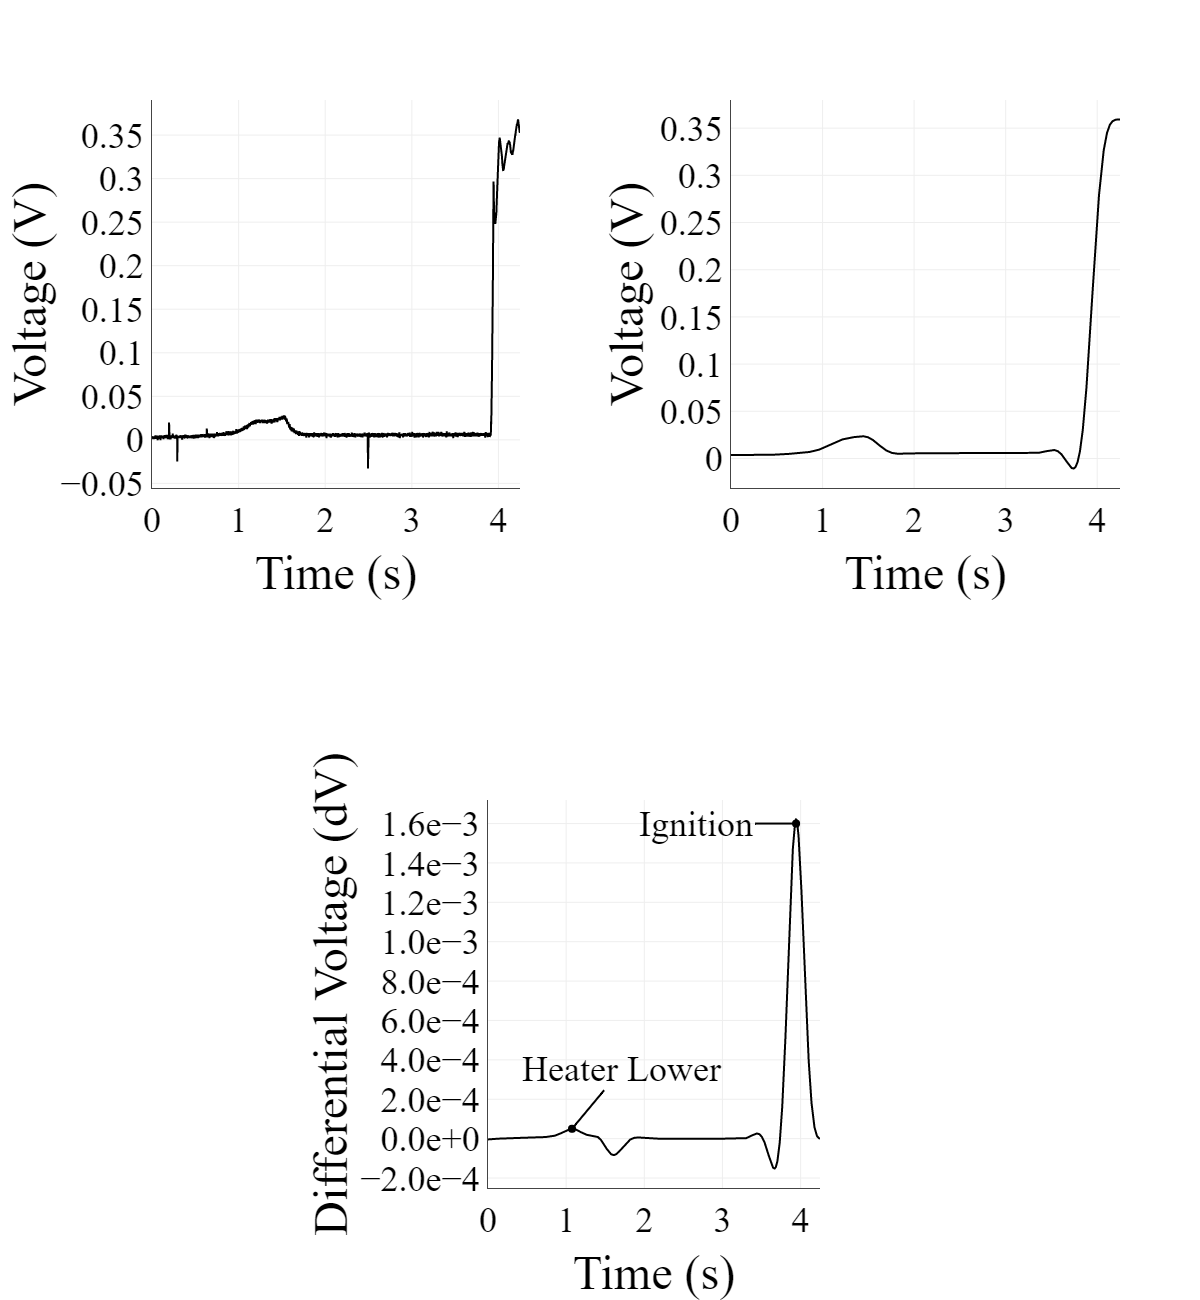
\includegraphics[width=\figureWidthSet]{Figures/stacked_photodiode.png}};
        %         \begin{scope}[x={(image.south east)},y={(image.north west)}]
        %             \node at (0.26, 0.5) {(A)};
        %             \node at (0.75, 0.5) {(B)};
        %             \node at (0.5, -0.03) {(C)};
        %         \end{scope}
        %     \end{tikzpicture}
        %     \end{center}
        %     \caption{Sample photodiode trace showing the signal in the three stages of analysis., \textbf{(A)} Raw Signal, \textbf{(B)} Filtered Signal, and \textbf{(C)} Signal Derivative}\label{fig:photoTrace}
        % \end{figure}

       
    The heat transfer to the fuel bed was estimated by applying an energy balance around the heater using the supplied (measured) power to the heater and subtracting the calculated infrared radiation losses to the surroundings. The heat flux was determined by normalizing the heat transfer to the heater by one-half of the surface area of the heater.  This surface area was justified as the heater was inserted to a depth of half the diameter for each test. Heat loss to the surroundings was estimated by measuring temperatures along the length of the heater but with no fuel bed material in the apparatus. These temperature profiles were then used to estimate the heat losses to the ambient. The emissivity of the heater was taken to be 0.60~\cite{Watlow2020}. Heat flux values were calculated as an average for the duration of the test, and for a 200\si{\milli\second} window when the heater made contact with the fuel bed. These two time scales allowed differences in sensitivities between average and initial heat flux to be observed. The heat flux values provide insights into variations in the characteristic rate of heat transfer from the heater to the fuel bed for each of the materials tested. Combining the heat flux for each material with the estimated thermal conductivity of the fuel bed enabled representative temperature distributions within the fuel bed to be determined. It is acknowledged that the processes addressed in this work are transient, thus the thermal diffusivity of the materials is applicable. However, thermal conductivity is considered here because the calculation of the thermal conductivity relies on fewer correlations and is potentially more accurate. Additionally, the thermal properties of the materials are derived from literature such that both properties are directly proportional to the experimentally obtained bulk density. Thermal conductivity of the fuel bed materials were estimated using the mean of minimum and maximum effective thermal conductivity correlations in porous media~\cite{bergman2011fundamentals}. The correlation for effective thermal conductivity is shown in Equation~\ref{eqn:estk} where $\epsilon$ is defined as the proportion of volume occupied by air, as is shown in Equation~\ref{eqn:epsilon}. 
        \begin{equation}
            k_{eff} = \frac{1}{2} \left(\frac{1}{\left( 1 - \epsilon \right)/k_{solid} + \epsilon/k_{air}} +  \epsilon k_{air} + \left(1-\epsilon \right) k_{solid} \right)
            \label{eqn:estk}
        \end{equation}
        \begin{equation}
            \epsilon = 1- \frac{\rho_{solid}}{\rho_{bed}}
            \label{eqn:epsilon}
        \end{equation}
    The thermal conductivity of Douglas-fir plates and corrugated cardboard plates were obtained from literature~\cite{Laboratory2010, Asdrubali2015}. The bulk density of the porous material ($\rho_{porous}$) and the solid ($\rho_{solid}$) were obtained from experimental samples. Table~\ref{tab:k_values} shows the mean bulk density for each material and the corresponding estimated thermal conductivity values for the porous materials and the solid plates. The values shown in Table~\ref{tab:k_values} were used as inputs to the computational models, as discussed later. 
        \rowcolors{2}{gray!25}{white}
        \begin{table}[hpbt]
            \caption{Measured ($\bar{\rho}$) and estimated (k) fuel bed properties}
            \centering
            \begin{tabular}{crr}
                \rowcolor{gray!50}
                Material & $\bar{\rho}$ (\si{\kilo\gram\per\cubic\meter}) & k (\si{\watt\per\meter\per\kelvin}) \\
                \hline
                Douglas-fir plates  & 510   & 0.120 \\
                $L_{c}<$1mm         & 135   & 0.042 \\
                4mm $<L_{c}<$ 6mm   & 69.9  & 0.034 \\
                6mm $<L_{c}<$ 12mm  & 36.9  & 0.030 \\
                Cardboard plates    & 115   & 0.053
            \end{tabular}
            \label{tab:k_values}
        \end{table}

    Three simplified models were implemented to obtain further insights into the physical and chemical processes causing trends observed in the experimental ignition efforts.
    First, the temperature evolution of the fuel bed was modeled. Second, the time-averaged mass flux and species concentrations of the pyrolysis species leaving the fuel bed and entering the air were estimated using the calculated temperatures of the fuel bed. Third, the ignition delay times of the gaseous pyrolysis species estimated to depart the fuel bed were calculated. Time-averaged and spatially constant values were used for mass flux and mass fraction of pyrolysis products leaving the fuel bed. Figure~\ref{fig:domains} shows the computational domain representing the fuel bed. Figure~\ref{fig:comp_flow} shows the data flow between the models where the rectangles indicate the implementation of a model or calculation, ellipses indicate an output of interest, and the rounded rectangles indicate an input from measurements or literature values. The dotted and dashed boxes outline which calculations pertain to each chemical mechanism used and the overlap shows the information that is transferred between the models. The fuel bed temperature was modeled using OpenFOAM~\cite{Foundation2020}. Modeling of the pyrolysis was conducted using Cantera~\cite{Goodwin2020} with the BioPOx mechanism~\cite{Dhahak2019}. The Bio1412 mechanism~\cite{Ranzi2008, Ranzi2001LumpingMixtures} was used for gas phase species exiting the fuel bed. The Bio1412 mechanism contains 137 species and 4533 reactions. The BioPox mechanism contains 710 species, 5035 reactions and includes both primary pyrolysis and secondary pyrolysis. The inclusion of secondary pyrolysis is important for the combustion of products in the fuel beds studied since the particle fuel beds contain air that may affect the composition of gases as they leave the fuel bed. 

        \begin{figure}
        \centering
        \resizebox{0.25\textwidth}{!}{%
          \begin{tikzpicture}
            \node at (0,0) (origin) {};
            \node at (40mm, 40mm) (topright) {};
            %\draw (origin) rectangle (topright);
            \draw [thick] (0mm, 40mm) -- (0mm,0mm) -- (40mm, 0mm) -- (40mm, 40mm);
            
            \fill [pattern=north west lines, pattern color= brown] (origin) rectangle (40mm, 40mm) node[pos=0.5] {Fuel Bed}; 
            \fill [draw=white,  inner color=red, outer color=white ] (20mm, 40mm) circle (10mm);
            \fill[fill=white] (8mm, 40mm) rectangle (32mm, 50mm);
            \filldraw [fill=white, draw=red, thick] (20mm, 40mm) circle (3mm);
            \draw [thick] (0, 40mm) -- (9mm, 40mm);
            \draw [thick, dashed] (9mm, 40mm) -- (17mm, 40mm);
            \draw [thick, dashed] (23mm, 40mm) -- (31mm, 40mm);
  
            \draw [thick](31mm, 40mm) -- (40mm,40mm);
            \fill[pattern=north east lines, pattern color=black!90] (-2mm,-2mm) rectangle (0mm,40mm) node[rotate=-90, pos=0.5] {};
            \fill[pattern=north east lines, pattern color=black!90] (0mm,-2mm) rectangle (40mm,0mm) node[rotate=-90, pos=0.5] {};
            \fill[pattern=north east lines, pattern color=black!90] (40mm, -2mm) rectangle (42mm,40mm) node[rotate=-90, pos=0.5] {};

            
            \draw[-stealth,decorate,decoration={snake,amplitude=1pt,pre length=0pt,post length=2pt}] (16mm, 35mm) -- ++(-1mm, 9mm);
            \draw[-stealth,decorate,decoration={snake,amplitude=1pt,pre length=0pt,post length=2pt}] (14mm, 37mm) -- ++(-1mm, 7mm);
            
            \draw[-stealth,decorate,decoration={snake,amplitude=1pt,pre length=0pt,post length=2pt}] (24mm, 35mm) -- ++(1mm, 9mm);
            \draw[-stealth,decorate,decoration={snake,amplitude=1pt,pre length=0pt,post length=2pt}] (26mm, 37mm) -- ++(1mm, 7mm);
            
            \draw [|-|] (0mm, -5mm) -- (40mm, -5mm) node[pos=0.5, below] {40mm} ;
            \draw [|-|] (-5mm, 0mm) -- (-5mm, 40mm) node[pos=0.5, left] {40mm} ;
          \end{tikzpicture}
          }
        \caption{Diagram of the computational domain where black lines indicate domain boundaries, and red lines are boundaries defined by the heater. The arrows denote flow of pyrolysis products from the fuel bed into the air above the fuel bed.}
        \label{fig:domains}
    \end{figure}
    % go through the flow chart and talk about all of the steps
   
    Modeling of the temperature evolution of the fuel bed was implemented to represent what occurs during the experiments. The domain size for the fuel bed was 40\si{\milli\meter} wide and 40\si{\milli\meter} in depth and ensured that wall effects did not influence the heat transfer over the 10\si{\second} of simulations. The 10\si{\second} time limit was chosen since the majority of experimental ignitions occurred before 10\si{\second}, as explained shortly. Additionally, it was observed in experiments that the fuel bed began to lose contact with the heater beginning near 10\si{\second}, potentially reducing the applicability of the model beyond this time. All sides of the fuel bed domain were treated as insulated, aside from the heater interface. The insulated sides and bottom of the domain are representative of experimental conditions, but the insulated top surface does not account for losses due to convection or radiation from the fuel bed materials.  Nonetheless the calculated temperature distribution within the fuel beds are expected to be valid because heat transfer is dominated by conduction. Reactions and mass loss are not considered in determining the temperature distributions of the fuel beds. Despite these limitations, the calculated temperature distributions provide insights into the mass of each fuel bed material that undergoes pyryolysis which in turn is used for understanding the experimental results.

        \begin{figure}
        \centering
         \resizebox{\figureWidthSet}{!}{%
        \begin{tikzpicture}[node distance=3cm and 1cm]
            \node (tbed) [draw, process, text width=2cm, text centered ] {Estimate $T_{bed}$};
            \node (qprime) [draw, terminal, above of=tbed] {$q\prime\prime_{heater}$};
            \node (kbed) [draw, terminal, right of=qprime] {$k_{bed}$};
            \node (ybed) [draw, terminal, right of=kbed] {$Y_{bed}$};
            \node (pchem) [draw, process, right of=tbed, text width=2cm, text centered] {Pyrolysis Chemistry};
            \node (aexit) [draw, ellipse, below of=tbed] {$A_{exit}$};
            \node (mflux) [draw, ellipse, right of=aexit] {$m^{\prime \prime}_{pyrolysis}$};
            \node (rhogas) [draw, ellipse, right of=mflux] {$\rho_{pyrolysis}$};
            \node (yprod) [draw, ellipse, right of=rhogas] {$Y_{pyrolysis}$};
            \node (vgas) [draw, ellipse, below of=aexit] {$V_{gaseous}$};

            \node (ygas) [draw, ellipse, below of=yprod] {$Y_{gaseous}$};
            \node (flowsim) [draw, process, left of = ygas, text width=2cm, text centered] {Ignition Delay Calculation};
            \node (tgas) [draw, ellipse, left of=flowsim] {$\tau_{gaseous}$};
            \node [fit=(tbed) (yprod) (mflux),draw,dotted, black, thick] (fuelfit) {};
            \node (FBM) [below left] at (fuelfit.north east) {Fuel Bed Model};
            \node [below] at (FBM.south) {(BioPOx)};
            \node [fit=(aexit) (vgas) (mflux) (tgas) (yprod) (flowsim),draw,dashed,black, thick] (gasfit) {};
            \node (QAM)[above] at (flowsim.north) {(Bio1412)};
            \node [above] at (QAM.north) {Gaseous Species Model};
            \draw [arrow] (kbed) -- (tbed);
            \draw [arrow] (qprime) -- (tbed);
            \draw [arrow] (tbed) -- (pchem);
            \draw [arrow] (tbed) -- (mflux);
            \draw [arrow] (tbed) -- (aexit);
            \draw [arrow] (kbed) -- (tbed);
            \draw [arrow] (ybed) -- (pchem);
            \draw [arrow] (pchem) -- (rhogas);
            \draw [arrow] (pchem) -- (yprod);
            \draw [arrow] (rhogas) -- (vgas);
            \draw [arrow] (mflux) -- (vgas);
            \draw [arrow] (aexit) -- (vgas);
            \draw [arrow] (yprod) -- (ygas);
            \draw [arrow] (flowsim) -- (tgas);
            \draw [arrow] (ygas) -- (flowsim);
        \end{tikzpicture}
        }
        \caption{Illustration of the model used for the estimated heater flux ($q_{heater}^{\prime \prime}$), thermal conductivity of the fuel bed ($k_{bed}$), and chemical composition of the fuel bed ($Y_{bed}$), (e.g., cellulose)  to calculate temperature ($T$) and pyrolyzate distribution above the fuel bed, and determine the resulting ignition delay times($\tau$). Here the subscript $bed$ represents the properties of the fuel bed materials and $pyrolysis$ represents the pyrolysis products leaving the fuel bed and entering the air above the fuel bed. For example, $V_{pyrolysis}$ represents the velocity of pyrolysis gases leaving the fuel bed and entering the quiescent air domain.}
        \label{fig:comp_flow}
    \end{figure}
    
     Combustion of the fuel bed materials was considered in two steps. Reactions occurring within the domain of the fuel bed were characterized with the BioPOx mechanism to include both pyrolysis and gas phase reactions. Reactions occurring at the exit of the fuel bed were considered solely gas phase, thus the Bio1412 mechanism was used. Chemistry calculations for both domains were performed in Cantera. A detailed chemistry model was considered to best capture the physics of the ignition process. However, a detailed discussion of differences in chemistry leading up to ignition are beyond the scope of this work. Instead, this work focuses on qualitative insights into ignition behavior. The mass of the fuel bed undergoing pyrolysis was defined as the mass of the fuel bed material above 220\si{\celsius}. 220\si{\celsius} was selected as it corresponds to the onset of hemicellulose pyrolysis~\cite{Yang2007} and is the lowest temperature estimated for reactions to occur encapsulating the potential breakdown of all constituents. The temperature at which pyrolysis occurred was taken as the average temperature of the fuel bed material above the temperature threshold. This step was necessary since the Cantera calculations performed were 0D. This approach provided an estimate of the average mass per unit time undergoing pyrolysis reactions. The exit area of the pyrolysis products was assumed to be constant for the duration of the test and was defined by the surface area of the fuel bed adjacent to the heater above the pyrolysis temperature at 10\si{\second}. Species were anticipated to depart the fuel bed and participate in gas phase reactions if they were included in both mechanisms. The mass flux of species departing the fuel bed was defined as the mass fraction of the gas phase species in the fuel bed relative to the mass of the fuel bed undergoing pyrolysis (T\textgreater220\si{\celsius}) divided by the surface area of the fuel bed above the pyrolysis temperature as shown by the dashed lines in Figure~\ref{fig:domains}. While in a physical experiment the mass flux and exit area would vary with time, all materials were treated equally in this study for simplicity and consistency in generating and understanding trends.
        
\section{Results}
   The time required for flaming ignition to occur for the various fuel beds is shown in Figure~\ref{fig:ignTime} as a function of heater set point temperature. Four observations are noted. First, the ignition times generally occurred  within the first 10\si{\second}.  If ignition did not occur after 10\si{\second} then it would typically take between 100\si{\second} and 1000\si{\second} to ignite, if at all. Conditions where ignition did not occur are not included in Figure~\ref{fig:ignTime}. A histogram of ignition times and the probability density for each material are shown in Figure~\ref{fig:ignHist} to further quantify the distribution of ignition times. The probability density of the $L_{c}<$ 1\si{\milli\meter} fuel particles, Douglas-fir plates, and cardboard plates are normally distributed with centers at 2.3\si{\second}, 2.8\si{\second}, and 3.9\si{\second}. The $L_{c}<$ 1\si{\milli\meter} fuel particles have an outlier peak centered at 1000\si{\second}. The 4\si{\milli\meter} $<L_{c}<$ 6\si{\milli\meter} and 6\si{\milli\meter} $<L_{c}<$ 12\si{\milli\meter} fuel particles are bimodal with highest density peaks at 1.7\si{\second} and 113\si{\second} respectively. The secondary peaks occur at 113\si{\second} for the 4\si{\milli\meter} $<L_{c}<$ 6\si{\milli\meter} fuel particles and 2.1\si{\second} for the 6\si{\milli\meter} $<L_{c}<$ 12\si{\milli\meter} fuel particles. Second, the probability of ignition at extended times increased as the particle sizes increased. Specifically, the proportion of ignition events in where $t_{ign} <$ 10\si{\second} group were 90\%, 77\%, and 47\% for the particles $L_{c}<$ 1\si{\milli\meter}, 4\si{\milli\meter} $<L_{c}<$ 6\si{\milli\meter}, and 6\si{\milli\meter} $<L_{c}<$ 12\si{\milli\meter} particle sizes, respectively. The third observation is that ignition was not observed beyond 100s for either of the solid plate fuel bed materials. Trends in ignition times for the plates were most similar to those for beds with the smallest particles. Fourth, for the ignition events that occurred within the first 10\si{\second} there is no apparent relationship between time to ignition, temperature, particle size, and fuel bed type. Additionally, the long timescales of some ignition events suggest that smoldering initiates and then transitions to flaming combustion. Since the incidence of ignition at extended times increases as the particle size increases the potential for smoldering to flaming transition is attributed to thermal and physical properties of the fuel bed. The different sensitivities of ignition just described are attributed to differences in the bulk thermal properties, the interface between the heater and fuel bed, and the global equivalence ratio of the fuel bed, as explained later. 
        \begin{figure}[htp]
            \centering
            \begin{tikzpicture}
                \node[anchor=south west,inner sep=0] (image) at (0,0) {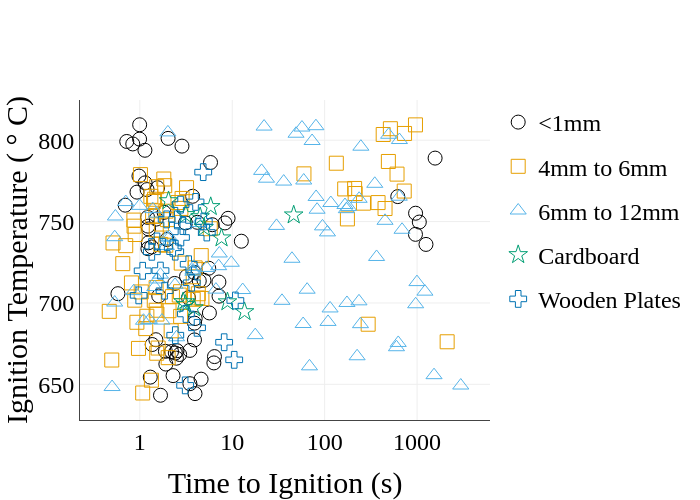
\includegraphics[width=\figureWidthSet]{Figures/ignition_comparison.png}};
                    \begin{scope}[x={(image.south east)},y={(image.north west)}]
                        \draw[dashed, thick,rounded corners] (0.12, 0.17) rectangle (0.33, 0.80);
                        \draw[dotted, thick,rounded corners] (0.46, 0.17) rectangle (0.68, 0.80);
                    \end{scope}
            \end{tikzpicture}
            % 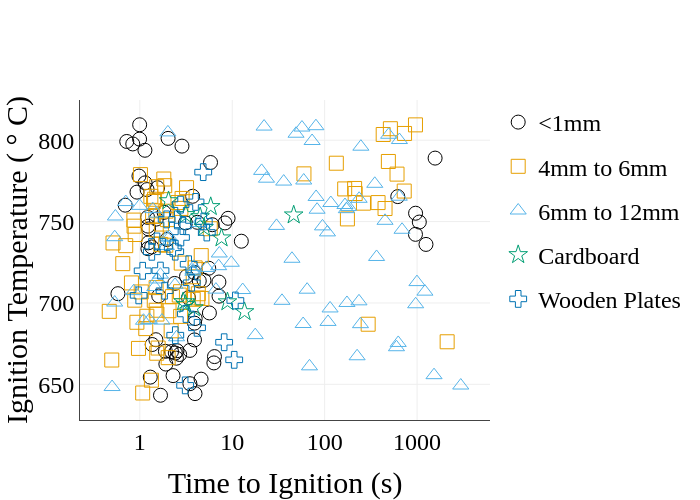
\includegraphics[width=\figureWidthSet]{Figures/ignition_comparison.png}
            \caption{Time to ignition and heater temperature at ignition for all fuel bed materials. 
            The dashed and dotted boxes emphasize the two general times-scales associated with ignition.}
            \label{fig:ignTime}
        \end{figure}
    

        \begin{figure}[htpb]
            \centering
                \begin{tikzpicture}
                \node[anchor=south west,inner sep=0] (image) at (0,0) {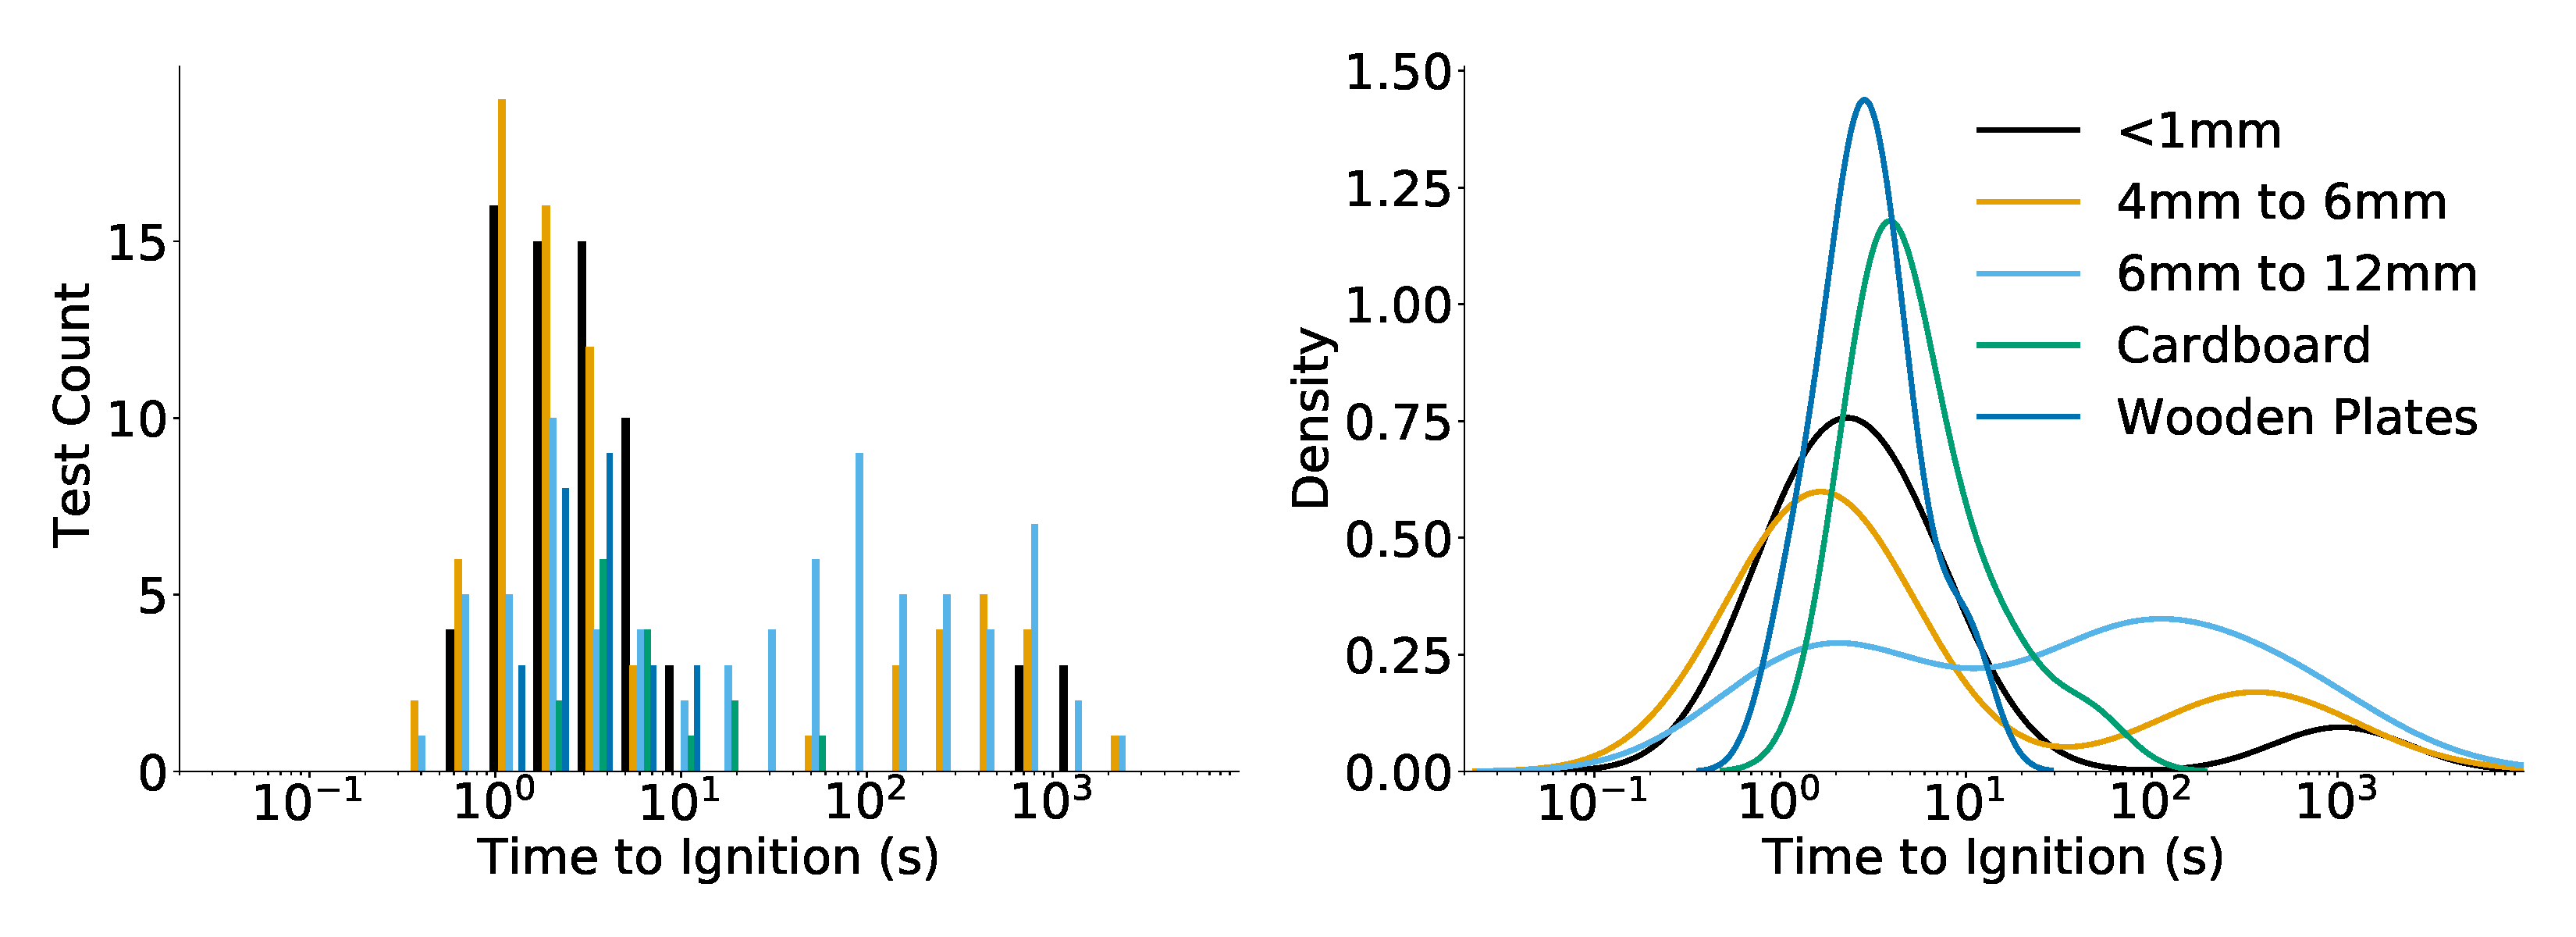
\includegraphics[width=\textwidth]{Figures/hist_and_kde.pdf}};
                    \begin{scope}[x={(image.south east)},y={(image.north west)}]
                        \draw[dashed, thick,rounded corners] (0.15, 0.185) rectangle (0.263, 0.9);
                        \draw[dotted, thick,rounded corners] (0.335, 0.185) rectangle (0.45, 0.52);
                        \draw[dashed, thick,rounded corners] (0.62, 0.185) rectangle (0.76, 0.9);
                        \draw[dotted, thick,rounded corners] (0.835, 0.185) rectangle (0.95, 0.52);
                    \end{scope}
            \end{tikzpicture}
            \caption{Ignition count (left) and probability density (right) of time to ignition for the fuel bed materials tested. The dashed and dotted boxes corresponding to the two zones of ignition from Figure~\ref{fig:ignTime}.}
            \label{fig:ignHist}
        \end{figure}
        
    The clustering of ignition times in either the $t_{ign} <$ 10\si{\second} or 100\si{\second}  $<t_{ign}<$ 1000\si{\second} time-scales is attributed to shifting of dominant heat transfer modes from conduction to radiation.  This shift occurs because of the heater fixture apparatus and the physical properties of the fuel beds. Initially, the heater and the fuel bed are in contact. The beds with larger particles have lower bulk densities; larger fractions of the fuel bed consist of air and have less contact area between particles. As a result, the effective thermal conductivity of the fuel beds decreases as the particle size increases as is shown in Table~\ref{tab:k_values}. For a fixed heater temperature the higher effective thermal conductivity for the smaller particles would result in a higher mass of particles above the pyrolysis temperature (as supported by calculations) producing conditions more conducive to ignition. As particle sizes decrease the pyrolysis products are also in closer proximity to the heater increasing the chances of either heating or piloted ignition as the gas flows over the heater. As a result, a larger percentage of smaller particle fuel beds ignite within 10\si{\second}, than the larger particle fuel beds (i.e., the second trend noted for Figure~\ref{fig:ignTime}). As heating progresses, a separation between the fuel bed and heater occurred because the heater was held in a fixed location while the fuel bed height decreased because of pyrolysis. Anecdotally this separation was observed to occur after $\approx$10\si{\second} for the various fuel beds. This separation causes the dominant mode of heat transfer to shift from conduction to infrared radiation. This change is significant because it corresponds to  ignition times to shifting from being less than 10\si{\second} to being generally greater than 100\si{\second}, as shown in Figure~\ref{fig:ignHist}. In addition, the larger particles tended to be longer thin particles which, on average, have a larger view factor per volume than the smaller particles. Hence, higher energy deposition per volume occurs for the larger particles when radiation is the dominant mode of heat transfer. As a result, the larger particle fuel beds more readily receive radiation and more readily ignite for $t_{ign} >$100\si{\second}, consistent with the trends discussed previously. The shift in dominant modes of heat transfer also causes solid plate fuel beds to not ignite after 100\si{\second}.  As separation between the heater and fuel occurs and heat transfer shifts to being dominated by radiation, the higher thermal conductivity of the solid materials (i.e., $k_{solid}=0.12$\si{\watt\per\meter\per\kelvin} vs $k_{<1mm} \approx 0.042$ \si{\watt\per\meter\per\kelvin}) reduces the temperature gradients, peak temperatures, and the release of pyrolyzates. 
    
    Further analysis of the time to ignition results reaffirm the influence of the fuel bed properties and heat transfer between the heater and fuel bed. A random forest regression model was implemented using the scikit-learn python package~\cite{scikit-learn} to identify which parameters were most correlated to the incidence of ignition occurring at either less than or greater than 10\si{\second}. The random forest regression model builds a series of independent decision trees based on experimental variables (e.g., average heat flux, particle size, etc.) and determines from those trees which variables have the largest influence on predicting the correct outcome (i.e., flaming ignition). A model is then assembled based on the specific values of each variable that best predict the desired outcome. Of the parameters recorded or calculated from experimental results, the incidence of ignition within each of the time scales was predicted with at least a 90\% certainty (out of bag and R$^{2}$ validation) when considering the estimated heat flux to the fuel bed, the fuel bed density, the power delivered to the heater at the time of heater contact, and the heater temperature. The power delivered to the heater at the time of heater contact is included as it serves as a comparison for a an initial reference of heat flux by which a comparison between ignitions that occurred in the radiation dominated mode at extended times which may bias the average heat flux values. The importance of these factors highlight the dependencies previously discussed in that the fuel bed properties and heat transfer to the fuel bed significantly influence the time-scales associated with ignition.  Moreover, the random forest analysis highlights a potential way that ignition may be predicted with a subset of information about the fuel bed. 
    
   The results and analysis just described focus on the characteristics of igniting cases; Figure~\ref{fig:ignProb} shows the probability of ignition for each of the fuel bed materials as a function of the heater temperature. The probability reported for each condition is based on the experiments being repeated at least five times.  In general, the ignition probability increased as the heater temperature increased, as expected because of the higher energy deposition. It is noted that as the heater temperature increases the potential for piloted ignition of pyrolysis gases increases. However, ignition occurs both above and below the piloted ignition temperature region and there is not a significant shift in trends at higher heater temperatures. This suggests that the influence of piloted ignition on the results is less significant than the increase of heat transfer rates to the fuel beds at higher temperatures. 
   
   When considering differences in ignition between fuel bed types the fuel beds with smaller particles typically had higher ignition probabilities at a temperature than beds with larger particles. At the lower temperatures, the plates tended to have lower ignition probabilities than the porous beds, but the plates transitioned from no ignition to unity ignition probability across a narrower range of temperatures than the porous fuel beds. It is noted that significant deviations from the overall trends (i.e., decreases in ignition probability) are apparent for the $L_{c}<$ 1\si{\milli\meter} particles at 675\si{\celsius} and 750\si{\celsius} and for the 6\si{\milli\meter} $<L_{c}<$ 12\si{\milli\meter} particles at 700\si{\celsius}. The cause of these deviations are unclear, but it is plausible the changes are caused by differences in ablation of the fuels and shifts in the dominant mode of heat transfer depending on the temperature.
        \begin{figure}[htpb]
            \centering
            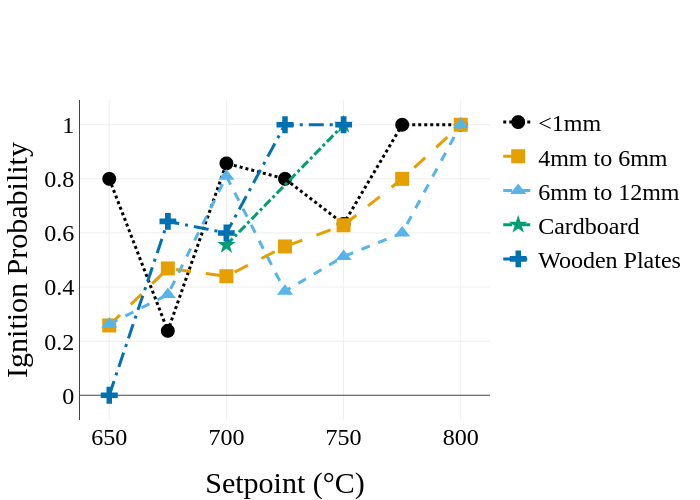
\includegraphics[width=\figureWidthSet]{Figures/setpoint_n5.png}
            \caption{Probability of ignition for each material as a function of heater set point temperature}
            \label{fig:ignProb}
        \end{figure}
    The sensitivities in ignition probability to the fuel bed characteristics, as shown in Figure~\ref{fig:ignProb}, are attributed to changes in area of the fuel bed in contact with the heater. Recall that the samples typically ignite within the first 10\si{\second}; hence conduction and the area of the fuel in contact with the heater are important in causing pyrolysis. As the particle size of the fuel bed increases fewer particles come into contact with the the heater, reducing the overall contact area. Additionally, the average distance between the heater and particles not in contact with the heater increases as particle size increases due to the reduced packing density of the particles. This may result in heat transfer from infrared radiation occurring over a more distributed volume within the fuel bed. As particle sizes increase the reduction in contact area and more distributed heat flux from radiation likely decrease the temperature gradient in the fuel bed as well as the local heat flux rates immediately adjacent to the heater, ultimately resulting in lower ignition probabilities for a fixed temperature as the particle size increases. 
    
    
    With regards to ignition of the Douglas-fir plates, it is expected that the solid materials behave similarly to the fuel beds with large particles (i.e., lower ignition probabilities at the lower temperatures) because the contact area between Douglas-fir plates and the cylindrical heater are more likely to be similar to the 6mm $<L_{c}<$ 12mm particles than the $L_{c}<$ 1mm particles. The Douglas-fir plates also have a much higher thermal conductivity and thermal mass than the particle fuel beds which is anticipated to result in similar temperature gradients between the largest particles and the plates. For the large particles infrared radiation to particles at greater distances from the heater, which would be occluded in the smaller particles, may act similarly to an increase in thermal conductivity and thus the similarity in ignition between the largest particles and Douglas-fir plates. The sharper transition from zero to unity ignition probability for the Douglas-fir plates is attributed to more consistent contact area between the heater and the plates from test to test. This uniformity is indicated in the narrower distribution of ignition times with only a $\approx$ 44\si{\second} difference between the shortest and longest ignition times for the Douglas-fir plates compared to $\approx$ 1550\si{\second} for the $L_{c}<$1mm particles. The narrower transition from non-ignition to ignition and the more consistent times to ignition of the Douglas-fir plates when compared to the particle fuel beds suggest that consistency in material properties and contact area between the heater and the fuel have a significant influence on ignition. 
    
    Similar to the time to ignition results, a random forest model was generated to gain insights into which parameters that are measured or derived are the most predictive of the occurrence of ignition of a fuel bed. The estimated heat flux to the fuel bed was the most influential parameter.  With the addition of the fuel bed density, heater temperature, and heat flux at contact with the fuel bed the prediction accuracy for ignition was 80\%.  These values were achieved based a 50\% test-train split of the entire dataset with out-of-bag and R$^{2}$ validation tests to measure predictive capabilities. The most noteworthy insight from this model is that the estimated average heat flux to the bed over the test duration has a much higher importance than the heater temperature for both porous and solid fuel beds. This is significant since the heat flux values, both upon contact and the overall average, encapsulate the effects of the heat transfer mode to the fuel bed unlike the surface temperature of the heater (or firebrand). A similar sensitivity of heat transferred to the fuel bed influencing ignition was observed by Fernandez-Pello et al.\cite{Fernandez-Pello2015}.
    
    Figure~\ref{fig:flux_comparison} shows the derived average heat fluxes to the fuel bed for each of the materials and heater temperatures tested. Results for igniting cases are represented by solid lines and non-igniting cases are represented with dashed lines. All the materials show two common trends except for cardboard plates, where not enough temperatures were evaluated to determine a trend. First, for tests where ignition occurred, and the heater setpoint was less than or equal to 750\si{\celsius} the heat flux to the fuel bed was higher than tests where ignition did not occur. Recall that the heater temperature is held constant, therefore variations in heat flux represent variations of heat transfer to the fuel. The implications of this are discussed in more detail later. Second, the heat flux values for tests where ignition occurred showed notable decreases in value for temperatures above 750\si{\celsius}, dropping lower than the values for the tests where ignition was not observed, in some cases.
        \begin{figure}[hbpt]
            \centering
            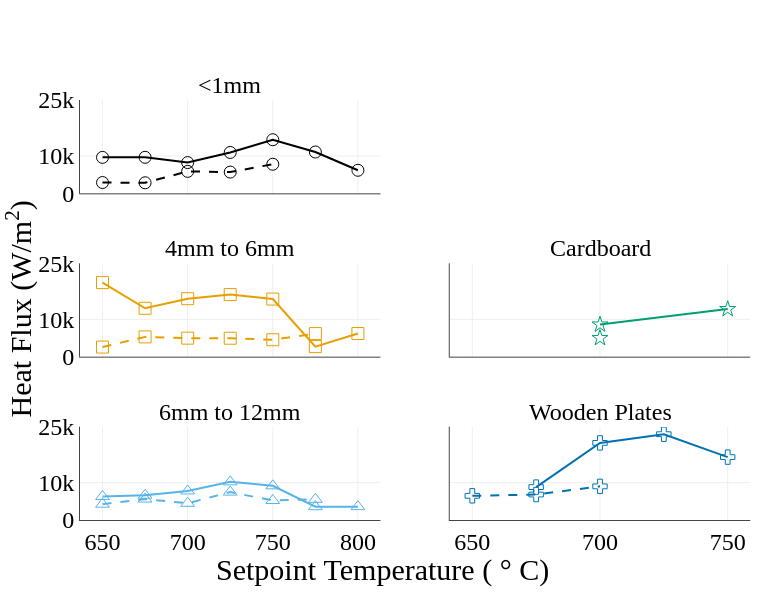
\includegraphics[width=\figureWidthSet]{Figures/power_comparison_trimmed.png}
            \caption{Comparison of estimated heat flux to the fuel bed for each material: dashed lines represents the mean of non-ignition tests and solid lines represent the mean of ignition tests for each heater temperature.}
            \label{fig:flux_comparison}
        \end{figure}
     Higher heat fluxes for the igniting cases compared to the non-igniting cases for the porous fuel beds are attributed to stochastic differences in contact area between the heater and the fuel bed particles. Seemingly, the tests with particles oriented in a manner that facilitates greater contact area have a higher heat flux due to increased conduction and are more likely to ignite. However, this assumption breaks down for high heater temperatures. At high heater temperatures (e.g., \textgreater750\si{\celsius}) the amount of heat transferred through infrared radiation appears be sufficient to counter differences in contact area and resulting conduction. Hence, this causes the reduction in the differences between igniting and non-igniting heat fluxes at the higher temperatures.  A sensitivity to the difference between igniting and non-igniting heat fluxes is noted depending on the particle sizes.  Specifically, in Figure~\ref{fig:flux_comparison}, the 4\si{\milli\meter} $<L_{c}<$ 6\si{\milli\meter} particles have greater differences in heat flux between the ignition and non-ignition cases when compared to the 6\si{\milli\meter} $<L_{c}<$ 12\si{\milli\meter} and $L_{c}$\textless1mm particles. The difference between igniting and non-igniting heat fluxes is correlated to the relative size of the particles compared to the diameter of the heater. For particles much smaller than the heater (\textless1\si{\milli\meter}) the random orientation of the particles would matter less than particles of similar size (4\si{\milli\meter} $<L_{c}<$ 6\si{\milli\meter}) as the heater. A similar phenomena is anticipated for particles larger than the heater (6\si{\milli\meter} $<L_{c}<$ 12\si{\milli\meter}), however, for the larger particles infrared radiation is anticipated to be more influential than conduction. Changes in contact between the heater and the fuel bed would then have a smaller effect on the rate of heat transfer as is shown by the spread in heat flux between ignition and non-ignition cases for the 6\si{\milli\meter} $<L_{c}<$ 12\si{\milli\meter} particles in Figure~\ref{fig:flux_comparison}. The 4\si{\milli\meter} $<L_{c}<$ 6\si{\milli\meter} particles appear to represent a near critical case where the conduction is still the driving heat transfer mode but variation in contact area is high producing a larger spread in heat flux.
     For the wooden plates a smaller number of heater temperatures with both ignition and non ignition heat flux values is observed suggesting test to test variation in contact area is not significant enough to prevent ignition.

    Results from OpenFOAM simulations of temperature profiles provide further insights into the effects of varying heat flux on ignition. Figure~\ref{fig:volumes} shows regions of the fuel bed above the pyrolysis temperature for (row I) a fixed 750\si{\celsius} boundary condition, (row II) a heat flux boundary condition based on the average values from ignition tests at the 750\si{\celsius}, and (row III) a heat flux boundary conditions based on  average heat fluxes for non-ignition tests at the 750\si{\celsius}. Column A shows the results for the fuel bed with $L_{c}<$ 1mm, column B with a bed of 4mm $<L_{c}<$ 6mm, and column C with a bed of 6\si{\milli\meter} $<L_{c}<$ 12\si{\milli\meter} particles. For the constant temperature boundary shown in row I, the region of the fuel bed above the pyrolysis temperature increases as particle sizes increase from left to right. Note, however, that the mass of the fuel bed material above the pyrolysis temperature decreases from left to right due to the decreasing density and thermal conductivity of the fuel bed as particle sizes increases. Specifically, the estimated mass of the fuel bed above the temperature for the onset of pyrolysis is 2.79\si{\micro\gram}, 1.59\si{\micro\gram}, and 1.55\si{\micro\gram} for columns (A), (B), and (C), respectively.  As a result, it is expected that the fuel bed with the smallest particles would release the most pyrolzates. 
    
    Perhaps surprising, is the difference in area at elevated temperatures between columns A and B in row II. Recall from Figure~\ref{fig:ignProb} that at this heater temperature (750\si{\celsius}) the particles with $L_{c}<$ 1\si{\milli\meter} (i.e., column A), and the 4\si{\milli\meter} $<L_{c}<$ 6\si{\milli\meter} (i.e., column B) have nearly identical ignition probabilities; however, the calculated average temperatures and region undergoing pyrolysis are notably different (e.g., 175\si{\celsius}).  More importantly, a 30\% mass increase in pyrolyzates occurs from $L_{c}<$ 1\si{\milli\meter} to 4\si{\milli\meter} $<L_{c}<$ 6\si{\milli\meter} conditions.  The corresponding ignition delay time, calculated using mass of pyrolyzates released and the average temperature of the pyrolysis region, was 0.5\si{\second} for the $L_{c}<$1\si{\milli\meter} gaseous products compared to 0.06\si{\second} for the 4\si{\milli\meter} $<L_{c}<$ 6\si{\milli\meter} products. The differences in ignition delay time results from differences in the average fuel bed temperature and in the global equivalence ratio as pyrolyzates are released. Physically, these ignition delay times correspond to the characteristics of the pyrolyzates exiting the fuel bed. The differences in ignition delay time would suggest that the particles with 4\si{\milli\meter} $<L_{c}<$ 6\si{\milli\meter} would ignite more readily, counter to the measured similar ignition probability.  Note, however, that the calculated velocity of the gaseous products also varies, specifically 4.3$\cdot10^{-3}$\si{\meter\per\second} for the $L_{c}<$1\si{\milli\meter} fuel compared to 2.6$\cdot10^{-2}$\si{\meter\per\second} for the 4\si{\milli\meter} $<L_{c}<$ 6\si{\milli\meter} fuel bed.  In short, consideration of both the ignition delay time and exit velocity of the gases maybe needed to more completely capture ignition probabilities.

    The Damkohler number (\textit{Da}), which represents the ratio of the transport to chemical times-scales, has been used previously to consider ignition behavior~\cite{Dai2013}, and is now considered to help evaluate ignition behavior.  In this work, the ratio of the heater diameter $D$ normalized by the product of the exit velocity ($V_{exit}$) and ignition delay time ($\tau$) were considered, to create a Damkohler number of ignition for porous beds. This analysis results in the non-dimensional values of 2.42, 4.04, and 7.66 for the smallest to largest particles (respectively) for the results just described in the previous paragraph. Note that the smaller the (\textit{Da}) the smaller the transport time (relative to chemical time-scale) and the less time that a parcel of reactants is near the high temperatures of the heater. In its limit, rectants may diffuse/advect away from the fuel prior to ignition.
        \begin{figure}[htpb]
            \centering
                \begin{tikzpicture}
                \begin{scope}[xscale=-1, yscale=1]
                    \node[anchor=south west,inner sep=0] (image) at (0,0) {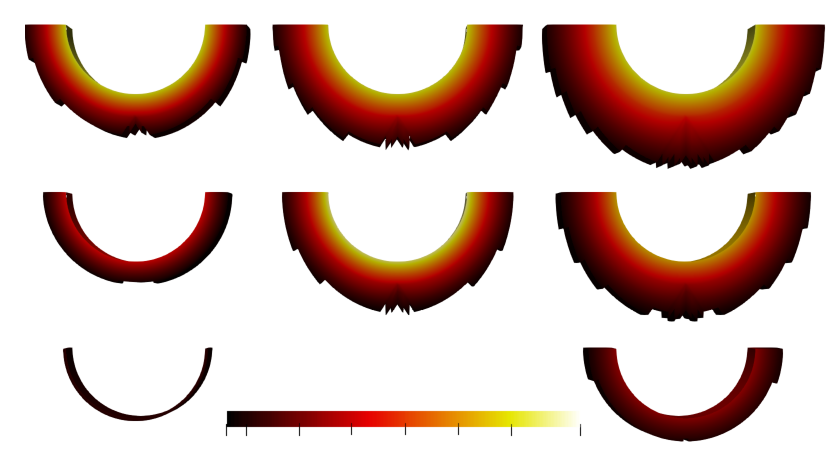
\includegraphics[width=\figureWidthSet]{Figures/fuel_bed_temperature_comparison_colorbar.png}};
                \end{scope}

                    \begin{scope}[x={(image.south east)},y={(image.north west)}]
                        \node at (-0.1, .82) {I};
                        \node at (-0.1, .5) {II};
                        \node at (-0.1, .15) {III};
                        \node at (0.16, -0.1) {A};
                        \node at (0.5, -0.1)  {B};
                        \node at (0.835, -0.1) {C};
                        \draw[dotted] (0, 0.64) -- (0.985, 0.64);
                        \draw[dotted] (0, 0.305) -- (0.985, .305);
                        \draw[dotted] (0, 0.045) -- (0.985, 0.045);
                        \draw[dotted] (0.30, 0.045) -- (0.30, 1);
                        \draw[dotted] (0.625, 0.045) -- (0.625, 1);
                        \draw[dotted] (0.985, 0.045) -- (0.985, 1);
                        \node at (0.27, 0.0) {220 (\si{\celsius})};
                        \node at (0.7, 0.0) {750 (\si{\celsius})};
                    \end{scope}
            \end{tikzpicture}
            \caption{Calculated region of fuel bed above the pyrolysis temperature 10\si{\second} after heater contact for a fixed  750\si{\celsius} boundary (I), ignition event heat flux (II), and non-ignition test event flux (III) for $L_{c}<$ 1mm (A), 4mm $<L_{c}<$ 6mm (B), and 6mm $<L_{c}<$ 12mm particles (C).}
            \label{fig:volumes}
        \end{figure}
    
    To further explore the potential role of using a (\textit{Da}) to characterize ignition propensity or porous, Figure~\ref{fig:nonDimPlot} shows the (\textit{Da}) number for the gaseous products at the exit of the fuel bed for each particle size and heater set point. Data from the plates is excluded, as the supporting calculations were beyond the scope of the work.  The abscissa is plotted relative to the average heat flux to the fuel bed multiplied by the thermal diffusivity of the fuel bed. These values were selected to include the influence of heat flux and thermal properties of the fuel beds in the characterization of ignition. Effectively, the chemical properties of the fuel bed and transport behavior are captured in the \textit{Da} analysis and thermal properties are included in the heat flux and thermal diffusivity. The lower right area of the plot, labelled No Ignition, represents values estimated to be less conducive to ignition (i.e., longer ignition delay times) than those observed to produce ignition in experiments. The region where ignition is expected contains the remainder of the plot and represents values estimated to equally or more conducive to ignition (i.e., higher heat fluxes and shorter ignition delay times) than those observed in experiments. The relative similarity trends in ignition behavior when considering the (\textit{Da}) indicate that considering the local transport conditions may be important to predicting ignition, in addition to considering the local heat flux and release of pyrolyzates. 
        
        \begin{figure}
            \centering
                            \begin{tikzpicture}
                \begin{scope}[xscale=-1, yscale=1]
                    \node[anchor=south west,inner sep=0] (image) at (0,0) {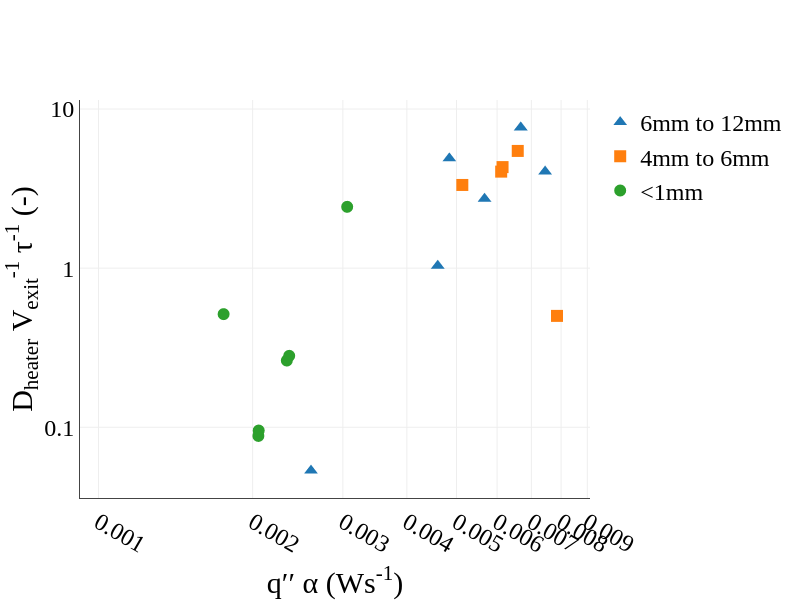
\includegraphics[width=\figureWidthSet]{Figures/ignition_trend.png}};
                \end{scope}

                    \begin{scope}[x={(image.south east)},y={(image.north west)}]
                        %   \fill[pattern=north east lines, pattern color=wongyellow, opacity=0.6] (0.1, 0.14) -- (0.73, 0.14) -- (0.73, .83) -- (0.6, 0.83) --cycle;
                         %\fill[pattern=north west lines, pattern color=wongorange, opacity=0.7] (0.40, 0.175) -- (0.73, 0.175) -- (0.73, .45) --(0.4, 0.45) --cycle;
                        \node at (0.567, 0.3) {No Ignition};
                    \end{scope}
            \end{tikzpicture}
            \caption{Comparison of non-dimensional chemical and flow timescale (for the igniting cases) as a function of heat flux time and thermal diffusivity. Conditions where ignition and non-ignition are anticipated are highlighted.}
            \label{fig:nonDimPlot}
        \end{figure}
    
    
   
\section{Summary and Conclusions}
    Flaming ignition tests have been conducted for porous Douglas-fir beds, Douglas-fir plates, and cardboard plates. A cylindrical cartridge heater was used as a firebrand surrogate. Heater temperature and electrical power to the heater were collected throughout each test. The derived heat flux to the fuel bed was within the range reported in literature of heat fluxes delivered by firebrands.  The time to ignition and probablity of ignition were used to evaluate the ignition propensity for the various fuel beds and heater temperatures.  A simplified heat transfer, pyrolysis, and ignition delay model was developed and used to provide further insights into the physical processes associated with ignition. The specific conclusions from this work are as follows.
        \begin{enumerate}
            \item 
                Smaller particles ignite more readily in porous beds than larger particles when heat transfer from the heater is primarily through conduction. This was evident by higher ignition probabilities, in general, of the smaller particles for a fixed heater temperature. As particle sizes increase radiant heat transfer becomes more important and fuel beds with larger particles were more likely than smaller particles to ignite at extended times (\textgreater 100\si{\second}) due to the increased importance of radiant ignition. 
            \item
                Douglas-fir plates ignite at times where conduction is the dominant mode of heat transfer (\textless 10\si{\second}) due to the higher thermal conductivity of the solid plates. The ignition probability of plates was the most similar to the larger particle, in particular at lower heater temperatures, due to dispersed heating of the porous fuel bed through radiation and the increased thermal conductivity of the plates creating similar temperature profiles. The rise in ignition probability  over a smaller heater temperature range time with temperature results from more consistent contact between the heater and plate surface.
            \item 
                Heat flux delivered to the fuel bed, when compared to heater temperature, is more indicative of ignition likelihood and ignition time for porous fuel beds. Heat flux is a more significant predictor of ignition because it captures differences in heat transfer modes and particle contact that heater temperature values do not. While this finding is not new, what is novel is that the mixed mode of heating (conduction and radiation) has a significant impact on the flaming ignition of fuel beds.
            \item 
                Consideration of the transport characteristics of pyrolyzate gases near the high temperature source can be important for more fully predicting ignition propensity. A \textit{Da} of ignition, in relation to the measured heat flux and thermal diffusivity of the fuel beds, is a promising relationship for predicting ignition for the porous fuel beds.  
        \end{enumerate}
    Further work is needed to verify that the \textit{Da} may be used to predict ignition for solid surfaces and for porous fuel beds with varying chemical compositions.  If proven valid, the (\textit{Da}), measured/predicted heat fluxes, and fuel bed properties may be used to help predict ignition of fuel beds both in and out of the WUI, ultimately helping to increase the effectiveness of fire prevention and suppression efforts.
